\documentclass[11pt]{article}
\usepackage{amsmath,amssymb,graphicx}
\usepackage[round]{natbib}
\usepackage{hyperref}
\usepackage{geometry}
\geometry{margin=1in}
\usepackage{graphicx}

\usepackage{tikz}
\usetikzlibrary{arrows.meta, positioning, shapes.geometric, fit, calc}

\title{From Behaviorism to Language Models: A Formal Correspondence Between the Matching Law and Token Prediction}
\author{Wesley R. Elsberry, Jory Schossau, Diane J. Blackwood, and Co-author N}
\date{\today}

\begin{document}
\maketitle

\begin{abstract}
We propose a formal correspondence between principles of operant behaviorism and the optimization dynamics of large language models (LLMs). The matching law, a cornerstone of behavior analysis, states that organisms allocate responses to alternatives in proportion to reinforcement rates. We demonstrate that this law parallels maximum likelihood estimation in LLM pretraining, generalized matching in reinforcement learning from human feedback (RLHF) and direct preference optimization (DPO), and temperature scaling at inference \citep{guo2017calibration}. Our framework is descriptive rather than normative: it identifies lawful allocation patterns across biological and artificial systems and provides testable predictions that move debate beyond metaphor.
\end{abstract}

\section{Introduction}
% [--- your edited Introduction here, unchanged ---]
The rise of large language models (LLMs) has intensified debate about
what, if anything, these systems learn. Some critics describe them as
“high‑tech plagiarism software” or “stochastic parrots,”
\footnote{The phrase ``stochastic parrot'' is in some sense more literally apt
for finite-order $n$-gram generators such as Emacs’s
\texttt{dissociated-press} or the \emph{Travesty} program published in
\emph{Byte Magazine} \citep{kenner1984travesty}. Our results show that contemporary LLMs
instantiate allocation laws that go beyond this baseline, though they do not by
themselves resolve questions of semantic grounding or bias.}
Some criticisms seem to emphasize
surface imitation over principle
\citep{bender2021dangers,chomsky2023nytimes}. Others argue that LLMs
demonstrate forms of generalization and adaptation that parallel
long-standing behavioral and cognitive theories. What is missing is a
formal framework that connects the optimization principles underlying
LLMs with the empirically validated laws of behavior established in
psychology.

In a different intellectual tradition, behavior analysis has long
emphasized lawful relations between environmental contingencies and
the allocation of behavior. One of the most influential contributions
of B.F. Skinner's radical behaviorism was the analysis of
\emph{selection by consequences}: behavior is shaped and maintained by
the contingencies of reinforcement in the environment
\citep{skinner1953science}. This perspective led to quantitative laws,
most prominently Herrnstein's matching law, which describes how
organisms allocate responses to alternatives in direct proportion to
reinforcement rates \citep{herrnstein1961matching}. Subsequent work
generalized this principle to account for systematic deviations in
sensitivity and bias \citep{baum1974generalized}.
Subsequent work generalized this principle to account for systematic deviations
in sensitivity and bias \citep{baum1974generalized}. The matching law continues
to be actively investigated and applied, from clinical interventions
\citep{kronfli2021matching}, to human communication behavior
\citep{anderson2024texting}, to neuroscience perspectives on reward expectations
\citep{rajagopalan2023reward}.

Modern LLMs are trained and aligned by equally precise optimization
principles. During pretraining, models minimize cross‑entropy and
therefore perform maximum‑likelihood estimation (MLE) to match
empirical token distributions. During alignment, objectives such as
RLHF and direct preference optimization (DPO) add a reward signal and
a KL regularization term against a reference model
\citep{christiano2017deep,ouyang2022training,rafailov2023direct}. At
inference, decoding procedures such as temperature sampling rescale
probabilities in a controlled way.
Although it is mathematically straightforward that idealized MLE recovers the
data distribution, interpreting this fact through the lens of the matching law
yields a cross-disciplinary insight: LLM token probabilities can be treated as
allocations of responses under contingencies.
This characterization does not anthropomorphize models; it identifies lawful
allocation dynamics that are substrate-independent (we refer to this as
\emph{allocation-grounding}). In effect, the corpus serves as the model’s
experiential channel: the structured set of contingencies from which allocations
are learned. We later describe this as a form of \emph{gestalt-grounding}, by
analogy to the sensory gestalt that shapes animal learning (see Discussion for
expansion upon this terminology of grounding types applicable to machine
learning).

Although reinforcement learning as a field has historical roots in psychology
and behaviorism \citep{sutton1998reinforcement}, the specific objectives used in modern LLM training and
alignment have been justified statistically rather than behavior-analytically;
to our knowledge, no prior work has shown their direct formal equivalence to
matching-law principles.


\textbf{Contributions.} We formalize and prove the correspondences
between: (1) MLE and strict matching; (2) KL‑regularized preference
optimization and generalized matching with interpretable sensitivity
and bias; and (3) temperature scaling and sensitivity rescaling. We
outline empirical tests and provide synthetic demonstrations. The
framework is descriptive, not normative: it clarifies how allocation
behaves under current training regimes, and it supplies testable
predictions that move discussion beyond metaphor.

At one level, the correspondences we present may seem almost obvious: learning
theory should apply whether the learner is a pigeon, a primate, or a program.
Yet, to our knowledge, prior discussions have relied largely on metaphor or
analogy rather than on formal correspondence. Our contribution is to replace
metaphor with proof: maximum-likelihood estimation instantiates strict matching,
KL-regularized alignment instantiates generalized matching, and temperature
scaling instantiates sensitivity rescaling. By showing that these well-known
optimization principles in machine learning are mathematically equivalent to
empirical laws in behavior analysis, we provide a framework that is at once
descriptively precise and empirically testable. This formalization, rather than
the intuition alone, is what makes the correspondence a novel advance.

\section{Related Work}
% [--- related work text here, unchanged ---]
Skinner’s \emph{Science and Human Behavior} \citep{skinner1953science} articulated a program in which reinforcement schedules and contingencies were sufficient to explain behavioral allocation without recourse to internal cognitive mechanisms. Building on this foundation, Herrnstein \citep{herrnstein1961matching} introduced the matching law, which formalized the observation that organisms allocate responses in proportion to the relative rates of reinforcement. Baum \citep{baum1974generalized} extended this into the generalized matching law, in which deviations from strict proportionality could be captured by parameters representing sensitivity and bias. Subsequent work in quantitative behavior analysis (e.g., \citealp{shimp1976short,grace1994temporal,killeen1994mathematical}) incorporated temporal dynamics, signal detection principles, and memory limitations. Despite this rich history, these principles have rarely been applied outside of biological behavior.

Associative models such as Rescorla and Wagner \citep{rescorla1972theory} provided mathematical descriptions of classical conditioning. Later, reinforcement learning frameworks (Sutton \& Barto, 1998) aligned these models with both machine learning algorithms and neural mechanisms of reward. Neuroscientific studies have shown that midbrain dopamine neurons encode reward prediction errors in ways consistent with operant formulations. Yet these literatures have remained largely confined to animals and humans, without systematic exploration of their relevance to large-scale language models.

Recent advances in artificial intelligence emphasize the role of scaling laws. Kaplan et al. \citep{kaplan2020scaling} demonstrated that model performance follows predictable power-law relationships with respect to parameters, data, and compute. At larger scales, qualitative changes emerge: Wei et al. \citep{wei2022emergent} documented emergent abilities such as zero-shot translation and reasoning. These studies highlight the predictive value of statistical regularities at scale but do not ground LLM behavior in pre-existing behavioral science frameworks.

Critical voices have questioned whether LLMs should be considered learners in any meaningful sense. Bender et al. \citep{bender2021dangers} described LLMs as “stochastic parrots,” generating outputs without understanding. Marcus \citep{marcus2022critique} has emphasized brittleness, lack of reasoning, and susceptibility to failure modes. Chomsky, Roberts, and Watumull \citep{chomsky2023nytimes} characterized LLMs as mere plagiarism systems, incapable of genuine insight. These critiques highlight the need for principled frameworks to describe what LLMs are doing, beyond metaphor or dismissal.

\paragraph{Relation to prior links with psychology.}
Reinforcement learning as a field has long drawn inspiration from behavioral and
cognitive psychology (e.g., Thorndike’s law of effect, Skinner’s operant
conditioning), and this lineage is acknowledged in foundational texts
\citep{sutton1998reinforcement}. However, the specific objectives that now
underlie large language model training and alignment---maximum likelihood
estimation, KL-regularized reinforcement learning from human feedback
\citep{christiano2017deep,ouyang2022training}, direct preference optimization
\citep{rafailov2023direct}, and temperature scaling \citep{guo2017calibration}---have
been justified in the machine learning literature primarily as statistical or
probabilistic principles. To our knowledge, no prior work has established a
direct formal correspondence between these objectives and the empirically
validated laws of allocation from behavior analysis, such as Herrnstein’s
matching law \citep{herrnstein1961matching} or Baum’s generalized matching law
\citep{baum1974generalized}. Our contribution is to make this correspondence
explicit and provable, replacing metaphor with formal equivalence.

Beyond its historical roots, the matching law remains a live area of research in
applied and theoretical contexts. Recent work has applied generalized matching
to evaluate treatment outcomes \citep{kronfli2021matching}, modeled operant
behavior in neural terms \citep{rajagopalan2023reward}, and extended allocation
analysis to everyday human activities such as texting
\citep{anderson2024texting}. Professional practice in applied behavior analysis
also continues to highlight matching law principles
\citep{mastermind2025matching}.

The present contribution is the first to systematically map
behavior-analytic principles---strict and generalized matching,
sensitivity, bias, and contextual constraints---onto the training and
inference of LLMs. By framing LLM outputs in terms of the matching
law, we re-situate their behavior as part of a broader class of
allocation phenomena observed in biological organisms. This does not
resolve all questions about generalization, compositionality, or
emergent abilities, but it does provide a benchmark descriptive
framework with which to analyze LLM performance.

\section{Formal Correspondence}
We summarize the main theoretical correspondences and provide statements sufficient for empirical testing.

\subsection{Notation and Setup}
Let $c$ denote contexts (prompts) and $y$ responses (tokens). Let $q(y\mid c)$ be the empirical next-token distribution, and $\pi_\theta(y\mid c)$ the model policy. The MLE loss is
\[
\mathcal{L}_{\text{MLE}}(\theta)=\mathbb{E}_{(c,y)\sim q}[-\log \pi_\theta(y\mid c)] = \mathbb{E}_{c\sim q}\big[H(q(\cdot\mid c),\pi_\theta(\cdot\mid c))\big].
\]
For KL-regularized RLHF/DPO at a fixed $x$, define
\[\mathcal{J}(\pi)=\mathbb{E}_{y\sim \pi(\cdot\mid x)}[r(x,y)]-\beta\,\mathrm{KL}(\pi(\cdot\mid x)\Vert \pi_{\text{ref}}(\cdot\mid x)).\]

\subsection{Theorem 1: Strict Matching under MLE}
\textbf{Statement.} If $q(\cdot\mid c)$ is representable, any global minimizer satisfies $\pi^{*}(\cdot\mid c)=q(\cdot\mid c)$; hence for $a,b$:
\[\frac{\pi^{*}(a\mid c)}{\pi^{*}(b\mid c)}=\frac{q(a\mid c)}{q(b\mid c)}.\]
\textbf{Sketch.} $H(q,\pi)=H(q)+\mathrm{KL}(q\Vert \pi)$ is minimized iff $\pi=q$.

\subsection{Theorem 2: Generalized Matching under KL-RLHF/DPO}
\textbf{Statement.} The optimizer of $\max_\pi \mathbb{E}_{\pi}[r]-\beta\,\mathrm{KL}(\pi\Vert\pi_{\text{ref}})$ is
\[\pi^{*}(y\mid x)\propto \pi_{\text{ref}}(y\mid x)\exp\{\beta r(x,y)\}.\]
Therefore
\[\log\frac{\pi^{*}(y_1\mid x)}{\pi^{*}(y_2\mid x)}=
\log\frac{\pi_{\text{ref}}(y_1\mid x)}{\pi_{\text{ref}}(y_2\mid x)}+\beta\,[r(x,y_1)-r(x,y_2)].\]
This realizes generalized matching with bias from $\pi_{\text{ref}}$ and sensitivity $s=\beta$.

\subsection{Theorem 3: Temperature Scaling}
Sampling with temperature $T>0$ rescales logits, giving $\pi_T(y\mid x)\propto \pi(y\mid x)^{1/T}$ and thus
\[\log\frac{\pi_T(y_1\mid x)}{\pi_T(y_2\mid x)}=\frac{1}{T}\log\frac{\pi(y_1\mid x)}{\pi(y_2\mid x)}.\]

\subsection{Theorem 4: Mixtures and Regularization}
If $q=\sum_k \alpha_k q^{(k)}$, then under capacity $\pi^{*}=q$ and pairwise odds follow mixture odds. Regularizers that shrink logits (KL to $\pi_{\text{ref}}$, label smoothing, entropy bonuses) attenuate log-odds (undermatching).

\section{Methods}
We describe empirical tests that operationalize the theoretical correspondences using standard corpora and open‑weight LLMs.

\textbf{Corpus–model matching (strict matching).} Select contexts \(c\) from a held‑out corpus (e.g., Wikipedia) and candidate continuations \(a,b\) with sufficient counts. Estimate \(\hat q(y\mid c)\) by relative frequencies and query pretrained models for \(\log \pi(y\mid c)\). Regress \(\log\frac{\pi(a\mid c)}{\pi(b\mid c)}\) onto \(\log\frac{\hat q(a\mid c)}{\hat q(b\mid c)}\). Prediction: slope \(s\approx1\), intercept \(\alpha\approx0\); finite‑capacity and finite‑sample effects produce systematic undermatching.

\textbf{Alignment tuning (generalized matching).} Starting from a base model and reference policy \(\pi_{\text{ref}}\), perform DPO or PPO‑style RLHF at a range of KL weights \(\beta\). For preference pairs \((y_1,y_2)\) given fixed \(x\), theory predicts
\[\log\frac{\pi(y_1\mid x)}{\pi(y_2\mid x)}=\log\frac{\pi_{\text{ref}}(y_1\mid x)}{\pi_{\text{ref}}(y_2\mid x)}+s\,[r(x,y_1)-r(x,y_2)],\]
with \(s=\beta\). Estimate \(s\) and test linearity and goodness‑of‑fit.

\textbf{Temperature scaling.} For a fixed model, vary sampling temperature \(T\in\{0.5,1,1.5,2,3\}\) and re‑estimate slopes \(s_T\) in the same log‑odds regressions. Prediction: \(s_T=s/T\).

\textbf{Mixture corpora and regularization.} When training on mixtures \(q=\sum_k \alpha_k q^{(k)}\), strict matching implies odds follow mixture odds; verify with small models. Test label smoothing and entropy bonuses, which should attenuate log‑odds (undermatching).

\textbf{Reproducibility.} Report slopes, intercepts, \(R^2\), and confidence intervals. Release scripts for corpus handling, model queries, and regressions. Synthetic figures here are proof‑of‑principle; empirical validation on open‑weight models is planned.

\subsection*{Synthetic Prototypes}

We include synthetic demonstrations to illustrate the correspondence between
machine learning objectives and matching-law principles in simplified settings.
These prototypes serve two purposes. First, they highlight
\emph{allocation-grounding}: the lawful and substrate-independent relation
between contingencies and allocations. For example, a toy model minimizing
cross-entropy over binary outcomes exhibits strict matching of allocation
ratios to reinforcement ratios. Second, they highlight
\emph{gestalt-grounding}: the role of the experiential channel in constraining
what contingencies are available to the learner. For example, limiting the
context window length in a synthetic text model produces systematic
undermatching, analogous to perceptual bandwidth limits in animal experiments.

The value of synthetic prototypes lies not in their realism but in their
clarity. By controlling all parameters, they make it transparent how allocation
laws emerge from optimization objectives, and how deviations can be diagnosed
as bias, sensitivity change, or gestalt constraint. This provides a baseline
against which both animal behavior and large-scale LLMs can be compared.

\subsection{Results: Synthetic Prototypes}
\begin{figure}[ht]
  \centering
  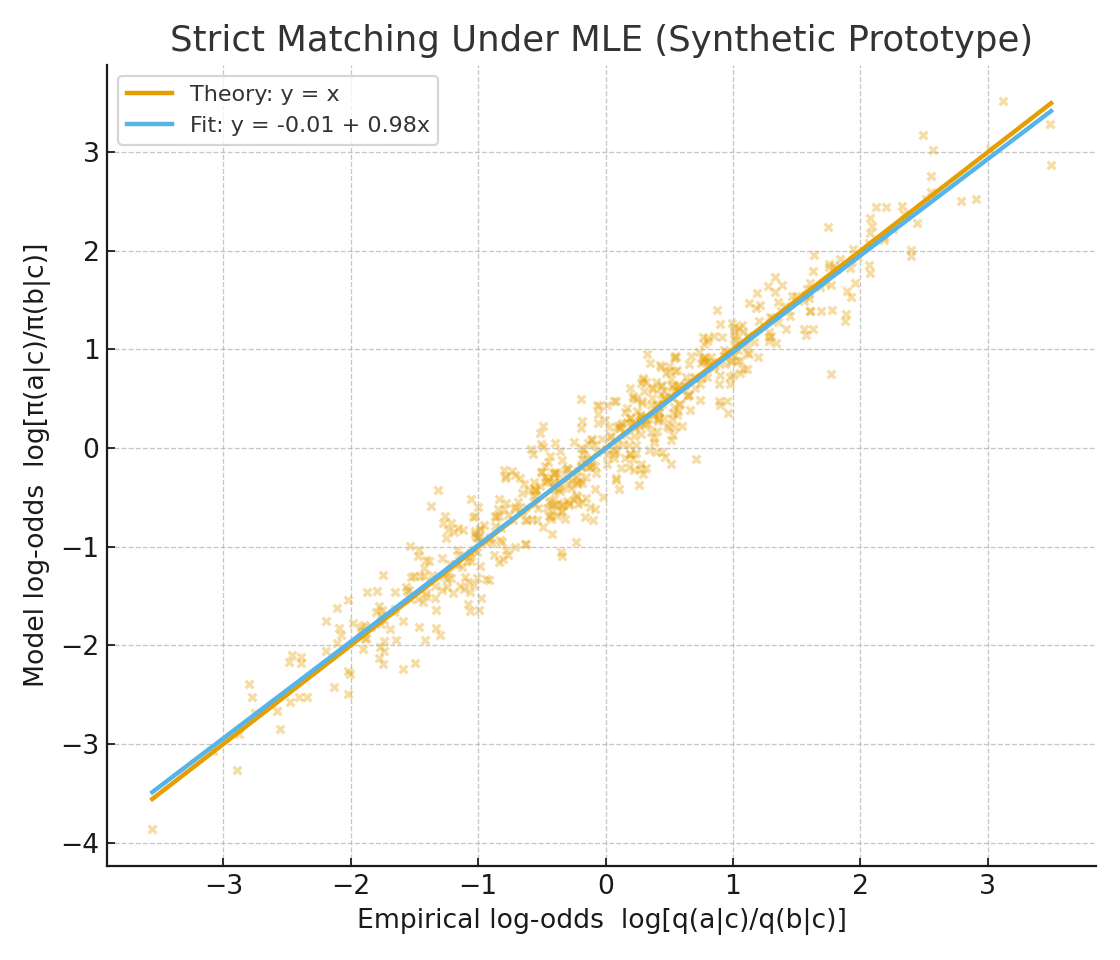
\includegraphics[width=0.65\textwidth]{figure2_strict_matching.png}
  \caption{Strict matching under maximum-likelihood pretraining.}
  \label{fig:strict}
\end{figure}

\begin{figure}[ht]
  \centering
  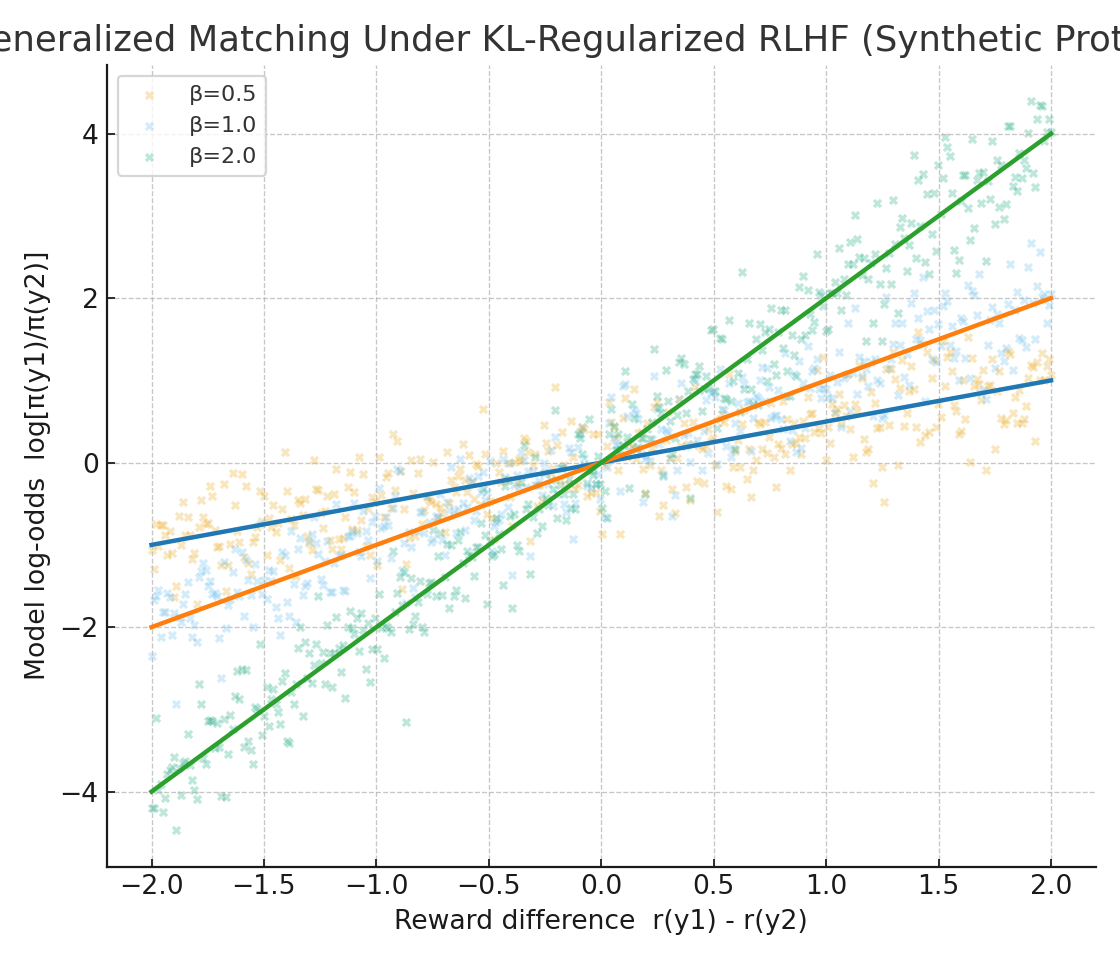
\includegraphics[width=0.65\textwidth]{figure3_generalized_matching.png}
  \caption{Generalized matching under KL-regularized RLHF/DPO.}
  \label{fig:gen}
\end{figure}

\begin{figure}[ht]
  \centering
  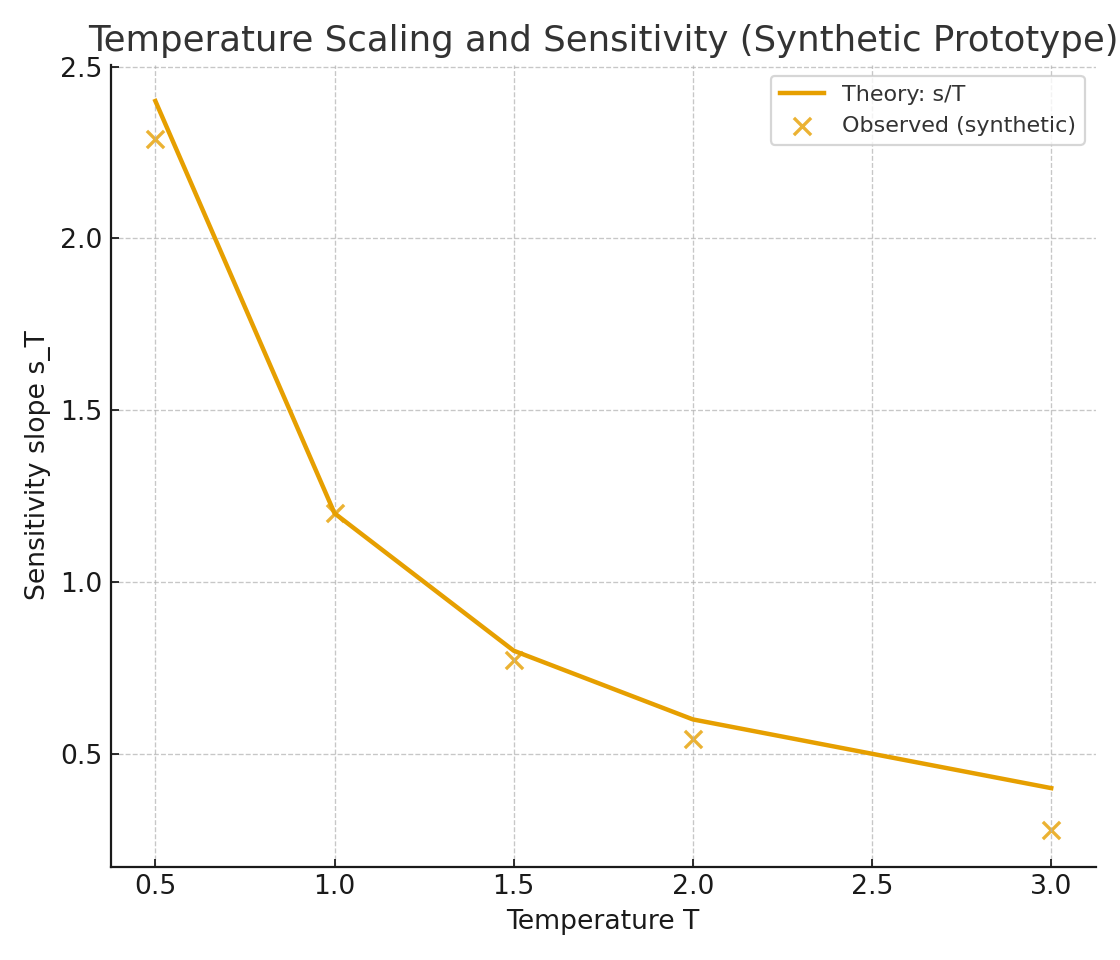
\includegraphics[width=0.65\textwidth]{figure4_temperature_scaling.png}
  \caption{Temperature scaling effects on sensitivity.}
  \label{fig:temp}
\end{figure}


\section{Empirical Program}

While our formal correspondences establish a descriptive framework,
empirical validation is essential. We therefore outline a program of
experiments at two levels: \emph{minimum viable demonstrations} and
\emph{optional extensions}.

\subsection{Minimum Viable Demonstrations}

\begin{enumerate}
  \item \textbf{Strict Matching Regression} \\
  Compute token-level logits from a pretrained model (e.g., GPT-2 small).
  Compare relative logit ratios for token pairs against empirical corpus
  frequencies. Demonstrate linear correspondence consistent with
  Herrnstein’s strict matching law.

  \item \textbf{Generalized Matching via Alignment} \\
  Fine-tune a small model with direct preference optimization (DPO) on a
  curated preference dataset. Fit generalized matching parameters
  (sensitivity, bias) to observed allocation shifts. Show that
  KL-regularization behaves analogously to generalized matching in
  animal choice.

  \item \textbf{Temperature Scaling} \\
  Generate outputs from a pretrained model at different sampling
  temperatures. Fit slopes of allocation curves to verify rescaling of
  sensitivity.
\end{enumerate}

These three experiments together suffice to demonstrate that
reinforcement-allocation principles hold across pretraining, alignment,
and inference.

\subsection{Optional Extensions}

\begin{itemize}
\item \textbf{Scaling Across Model Sizes} \\
  Replicate strict matching regression with models from 124M to 7B
  parameters. Assess whether sensitivity to corpus statistics improves
  with scale, paralleling quantitative shifts in animal matching across
  species.

\item \textbf{Memory and Context Constraints} \\
  Evaluate strict matching at varying context window lengths. Test the
  hypothesis that longer windows yield closer adherence to corpus
  contingencies, paralleling working-memory effects in animals.

\item \textbf{Comparative Datasets} \\
  Apply the same analyses to corpora with distinct statistical profiles
  (e.g., natural text vs. synthetic reinforcement schedules). Assess
  robustness of the correspondence.
\end{itemize}

\subsection{Summary}
The \emph{minimum program} (strict matching, generalized matching,
temperature scaling) establishes the core claim of a formal
correspondence. The \emph{optional extensions} provide depth, linking
allocation fidelity to model size, memory, and context --- and thereby
positioning LLMs more explicitly within the comparative framework of
behavioral science.

\section{Broader Research Program}
\label{sec:program}

The correspondences we have established are not merely conceptual. They yield
testable predictions and point toward an empirical program that bridges behavior
analysis and machine learning. This program has two complementary strands:
allocation-grounding (substrate-independent laws of matching) and
gestalt-grounding (substrate-specific constraints of perception or corpus).
The
particular contingencies that a system encounters depend on its
gestalt---sensory in organisms, textual in LLMs---so
allocation-grounding and gestalt-grounding are complementary rather than
contradictory perspectives. 

\subsection*{Cross-Cutting Standards}
To ensure comparability across models and organisms, we recommend reporting:
\begin{itemize}%[leftmargin=*]
  \item sensitivity (slope) and bias (intercept) from log-odds regressions;
  \item $R^2$ with confidence intervals;
  \item sample size, context granularity, and effective context length;
  \item regularization and decoding parameters (KL weights, temperature, top-$k$, $p$, repetition penalties);
  \item corpus domain or sensory channel (textual vs.\ perceptual gestalt \citep{koffka1935principles})
\end{itemize}

\subsection*{Core Tracks}
\paragraph{Track A: Allocation Benchmarks.}
Replicate strict matching (MLE), generalized matching (KL-regularized alignment), and temperature scaling on small LLMs and animal models.  
\emph{Milestone:} slopes near predicted values with interpretable bias.

\paragraph{Track B: Capacity and Gestalt.}
Vary context window (LLMs) or sensory bandwidth (organisms) to probe gestalt constraints.  
\emph{Milestone:} undermatching increases with reduced window/bandwidth; sensitivity improves with expanded gestalt.

\paragraph{Track C: Comparative Phenomena.}
Test classical conditioning \citep{rescorla1972theory} and in-context learning \citep{brown2020language} analogs.  
\emph{Milestone:} recovery of cue–outcome learning curves, blocking, and observational-learning analogs.

\paragraph{Track D: Mechanistic Probes.}
Investigate how embeddings (LLMs) or neural circuits (organisms) implement allocation adjustments.  
\emph{Milestone:} correlation between representational change and shifts in sensitivity/bias.

\subsection*{Program Matrix}
Table~\ref{tab:program} provides a mapping from behavioral constructs to LLM
mechanisms and specifies minimal and stretch experiments. Importantly, each row
can be interpreted through both allocation-grounding and gestalt-grounding:
allocation laws define what patterns to expect, while gestalt constraints define
what contingencies are accessible to the learner.

\subsection*{Risks and Mitigations}
\emph{Data bias:} stratify by domain; \emph{Overfitting to proxies:} validate
on held-out corpora and alternate tokenizations; \emph{Temperature/filters:}
report full decoding stack; \emph{Comparability:} match stimulus domain to
gestalt channel.

\subsection*{Artifacts and Reproducibility}
Release code, prompts, and corpora slices; provide CSVs with per$-$pair odds,
slopes, intercepts, and CIs; include model hashes and, for animal studies,
apparatus schematics. This ensures cumulative science across both allocation and
gestalt dimensions.

\subsection*{Summary}
The research program moves discussion beyond metaphor by embedding LLMs in the
same empirical cycle long used in behavior analysis: specify contingencies,
measure allocations, test laws, and interpret deviations. Allocation-grounding
supplies the general lawfulness; gestalt-grounding specifies the substrate that
enables or constrains it.


\begin{table}[h!]
\centering
\begin{tabular}{|p{0.22\textwidth}|p{0.34\textwidth}|p{0.34\textwidth}|}
\hline
\textbf{Row} & \textbf{Research Questions} & \textbf{Minimal Tests / Stretch Goals} \\
\hline
Operant $\leftrightarrow$ MLE (strict) &
Context granularity where strict matching holds? &
\emph{Minimal:} Log-odds regressions on held-out corpora; slope $\approx 1$, intercept $\approx 0$. \newline
\emph{Stretch:} Multi-token alternatives; compositional continuations; multilingual corpora.\\
\hline
Generalized matching $\leftrightarrow$ KL-alignment &
Map $\beta$ to sensitivity across datasets/models? &
\emph{Minimal:} DPO with $\beta$ sweep; fit slope/bias from log-odds shifts. \newline
\emph{Stretch:} PPO-style RLHF; compare to animal sensitivity estimates.\\
\hline
Inference temperature &
How stable is $1/T$ scaling across prompts/models? &
\emph{Minimal:} Temperature sweep; recover slopes $1/T$. \newline
\emph{Stretch:} Adaptive temperature; task-conditioned sensitivity.\\
\hline
Classical $\leftrightarrow$ supervised &
Do cue–outcome learning curves match associative models? &
\emph{Minimal:} Train small nets on cue–outcome pairs; fit Rescorla–Wagner-like curves. \newline
\emph{Stretch:} Blocking/overshadowing analogs in pretraining slices.\\
\hline
Hebbian $\leftrightarrow$ self-supervised reps &
Are updates consistent with correlation-driven rules? &
\emph{Minimal:} Track embedding changes under masked-LM objectives. \newline
\emph{Stretch:} Compare with neuro data (STDP-like signatures).\\
\hline
Observational $\leftrightarrow$ in-context &
How do demonstrations shape one-shot generalization? &
\emph{Minimal:} Prompt with examples; measure performance vs.\ number of demos. \newline
\emph{Stretch:} Sample-efficiency laws; compare to animal imitation.\\
\hline
Memory constraints $\leftrightarrow$ context windows &
How does allocation fidelity scale with window length? &
\emph{Minimal:} Strict matching vs.\ window size. \newline
\emph{Stretch:} External retrieval as “extended working memory”; quantify gains.\\
\hline
\end{tabular}
\caption{Expanded research program connecting behavior-analytic constructs to LLM mechanisms. Report sensitivity (slope), bias (intercept), $R^2$, and confidence intervals; include recency and capacity bounds where relevant.}
\label{tab:program}
\end{table}

\section{Discussion}
% [--- discussion text including memory/context subsection and figure ---]
The formal results show that core principles of operant psychology apply to LLM behavior at the level of allocation. Pretraining under MLE yields strict matching in the idealized limit; alignment with KL‑regularized reward yields generalized matching; temperature rescales sensitivity. These correspondences provide a compact language for expressing how model behavior changes across training and decoding settings.

\textbf{Relation to ``stochastic parrots.''}
Bender et al.\ (2021) introduced the metaphor of ``stochastic parrots'' to
highlight concerns about large-scale next-token prediction, including risks of
bias amplification, ecological costs, and questions about meaning. We agree
that these are serious considerations for responsible deployment. At the same
time, our results clarify that modern LLMs differ formally from literal
shufflers of surface statistics. Whereas finite-order $n$-gram generators
produce outputs by local concatenation with no global allocation principle,
contemporary LLMs are trained by objectives that yield allocation dynamics
consistent with the matching law. From a behavior-analytic perspective, this
constitutes a kind of grounding: models adapt allocations in proportion to
contingencies, in the same sense that organisms adapt behavior to experiential
reinforcement. Thus, while LLMs do not possess symbolic reference in the
classical semantic sense, they are not ungrounded; their ``semantics'' are
embodied in learned allocations. This distinction separates them sharply from
genuine parroting baselines (see Table~\ref{tab:ngram_vs_llm} and
Appendix~\ref{app:ngram} for code and examples).

\textbf{On “stochastic parrots” and plagiarism.} Saying that a model “repeats its training data” redescribes strict matching: allocations follow contingencies. The scientifically interesting question is how and when models \emph{deviate}—bias and undermatching quantify the impact of regularization, data mixture, and architectural limits. These deviations are diagnostic of learning structure rather than evidence of mere parroting.

\subsection*{What Kind of Grounding Do LLMs Provide?}

A central critique associated with the ``stochastic parrot'' metaphor is that
large-scale next-token prediction lacks semantic grounding. This assumes that
meaning requires symbolic reference to an external world model. From a
behavior-analytic perspective, however, grounding is not defined by internal
representational structures but by lawful adaptation of responses to
contingencies. In Skinner’s formulation, behavior is ``selected by
consequences''; allocation is grounded insofar as it tracks reinforcement in the
environment.

Our formal results show that LLMs instantiate precisely this kind of
allocation-grounding. During pretraining, maximum likelihood estimation drives
probabilities to match the distribution of linguistic contingencies in the
corpus. During alignment, KL-regularized objectives tilt allocations in
interpretable ways, analogous to sensitivity and bias in generalized matching.
At inference, decoding parameters such as temperature rescale these allocations
systematically. In each case, allocation is not arbitrary imitation but an
adaptive response to experienced contingencies.

Thus, while LLMs do not possess semantic grounding in the classical symbolic
sense, they are not ungrounded. Their semantics are \emph{operant semantics}:
meanings emerge as stable allocation patterns shaped by exposure and feedback.
This reframing clarifies why the ``stochastic parrot'' label, though apt for
$n$-gram generators, obscures what modern models actually achieve. LLMs are
grounded in their experience, much as organisms are grounded in reinforcement
histories, and this grounding can be formalized and tested using the matching
law correspondences. The broader empirical program we outline
(Table~\ref{tab:program}) specifies concrete experiments that make these
allocation-based grounding claims testable across scales, contexts, and
training regimes.

Importantly, these correspondences are not tied to obsolete
constructs. Matching law analysis is still a cornerstone of
contemporary behavioral research and application
\citep{kronfli2021matching,rajagopalan2023reward,anderson2024texting,mastermind2025matching},
demonstrating that the laws we connect to LLM objectives remain both
empirically and clinically robust.


%\begin{figure}[t]
%\centering
%\begin{tikzpicture}[
%  node distance=8mm and 12mm,
%  box/.style={rectangle, rounded corners, draw, align=center, inner sep=6pt},
%  small/.style={rectangle, draw, align=center, inner sep=4pt},
%  arr/.style={-{Stealth}, thick},
%  xarr/.style={-{Stealth}, thick, dashed},
%  lab/.style={font=\footnotesize},
%  title/.style={font=\bfseries}
%]
%
%% Column titles
%\node[title] (T1) {A. $n$-gram generator (finite-order Markov)};
%\node[title, right=45mm of T1] (T2) {B. LLM (training, alignment, inference)};
%\node[title, right=55mm of T2] (T3) {C. Operant organism (behavioral allocation)};
%
%% --- Column A: n-gram shuffler ---
%\node[box, below=5mm of T1] (A1) {Corpus counts \\ (local $n$-gram frequencies)};
%\node[box, below=of A1] (A2) {Fixed-order \\ Markov transitions};
%\node[box, below=of A2] (A3) {Local concatenation \\ (no global objective)};
%\node[box, below=of A3] (A4) {Output text};
%\node[small, below=of A4] (A5) {\textit{No allocation law}};
%
%\draw[arr] (A1) -- (A2);
%\draw[arr] (A2) -- (A3);
%\draw[arr] (A3) -- (A4);
%
%% --- Column B: LLM ---
%\node[box, below=5mm of T2] (B1) {Corpus $q(\cdot \mid c)$};
%\node[box, below=of B1] (B2) {Pretraining (MLE) \\ minimize $H(q,\pi)=H(q)+\mathrm{KL}(q\Vert \pi)$};
%\node[box, below=of B2] (B3) {Policy $\pi_\theta(\cdot \mid c)$ \\ \textit{strict matching in the limit}};
%\node[box, below=of B3] (B4) {Alignment (e.g., DPO/RLHF) \\ maximize $\mathbb{E}[r]-\beta\,\mathrm{KL}(\pi\Vert \pi_{\mathrm{ref}})$};
%\node[box, below=of B4] (B5) {Inference controls \\ temperature $T$, top-$k$/nucleus};
%\node[small, below=of B5] (B6) {\textit{Generalized matching:} \\ sensitivity $\sim \beta$ or $1/T$, bias $\sim \pi_{\mathrm{ref}}$};
%
%\draw[arr] (B1) -- (B2);
%\draw[arr] (B2) -- (B3);
%\draw[arr] (B3) -- (B4);
%\draw[arr] (B4) -- (B5);
%
%% --- Column C: Operant organism ---
%\node[box, below=5mm of T3] (C1) {Environmental contingencies \\ (reinforcement schedules)};
%\node[box, below=of C1] (C2) {Selection by consequences \\ (Skinner)};
%\node[box, below=of C2] (C3) {Behavioral allocation \\ $\displaystyle \frac{B_1}{B_2} \approx \frac{R_1}{R_2}$};
%\node[box, below=of C3] (C4) {Generalized matching \\ $\log\frac{B_1}{B_2}=\;s\,\log\frac{R_1}{R_2} + b$};
%\node[small, below=of C4] (C5) {\textit{sensitivity $s$, bias $b$}};
%
%\draw[arr] (C1) -- (C2);
%\draw[arr] (C2) -- (C3);
%\draw[arr] (C3) -- (C4);
%
%% --- Cross-column correspondences (dashed) ---
%\draw[xarr] ($(B2.east)+(0,0)$) .. controls +(1.6,0.3) and +(-1.6,0.3) .. (C3.west)
%  node[midway, above, lab] {strict matching (MLE $\Rightarrow \pi=q$)};
%\draw[xarr] (B4.east) .. controls +(1.6,0.0) and +(-1.6,0.0) .. (C4.west)
%  node[midway, above, lab] {KL-regularized $\leftrightarrow$ generalized matching};
%\draw[xarr] (B5.east) .. controls +(1.6,-0.3) and +(-1.6,-0.3) .. ($(C4.west)+(0,-0.1)$)
%  node[midway, below, lab] {temperature $T \Rightarrow$ sensitivity $1/T$};
%
%
%\end{tikzpicture}
%
%\smallskip
%\noindent\textbf{Legend / Mapping.}
%\begin{itemize}[leftmargin=1.2em]
%  \item \emph{n-gram:} finite-order Markov chain; no global optimization; “stochastic parrot” metaphor applies literally.
%  \item \emph{LLM Pretraining (MLE):} minimizes $H(q,\pi_\theta)=H(q)+\mathrm{KL}(q\Vert\pi_\theta)$; in the realizable limit, odds match (strict matching).
%  \item \emph{LLM Alignment (KL-regularized):} $\mathcal{J}(\pi)=\mathbb{E}[r]-\beta\,\mathrm{KL}(\pi\Vert\pi_{\mathrm{ref}})$ yields log-odds wi%h \textbf{bias} (from $\pi_{\mathrm{ref}}$) and \textbf{sensitivity} $\beta$ (generalized matching).
%  \item \emph{Decoding Temperature:} $\pi_T\propto\pi^{1/T}$; log-odds slopes scale with $1/T$ (sensitivity rescaling).
%  \item \emph{Operant organism:} allocation tracks reinforcement rates (matching law); deviations summarized by sensitivity and bias.
%\end{itemize}

% --- Legend ---
%\node[box, align=left, below=18mm of B6, minimum width=0.8\linewidth] (LEG) {%
%\textbf{Legend.}\;
%(A) $n$-gram pathway: finite-order Markov transitions from local counts; no global objective; \emph{parroting baseline}.\\
%(B) LLM pathway: MLE pretraining $\Rightarrow$ strict matching in the realizable limit; alignment with KL to reference $\Rightarrow$ bias/sensitiv%ity control; inference temperature rescales sensitivity.\\
%(C) Operant pathway: environmental contingencies $\Rightarrow$ allocation of behavior (matching law); generalized matching with sensitivity $s$ an%d bias $b$.};


%\caption{Parallel pathways and correspondences. $n$-gram generators (A) “parrot” local statistics without an allocation law. LLMs (B) implement global objectives whose allocation dynamics correspond to strict and generalized matching; temperature modulates sensitivity. Operant organisms (C) allocate behavior according to reinforcement schedules (matching law). Dashed arrows highlight formal analogies.}
%\label{fig:schematic_parrot_llm_operant}
%\end{figure}



% # 2
% ---- Add to preamble (once) ----

% ---- Figure in body ----
%\begin{figure}[t]
%\centering
%\begin{tikzpicture}[
%  node distance=8mm and 12mm,
%  >={Stealth},
%  box/.style={draw, rounded corners=2pt, align=center, inner sep=4pt, outer sep=2pt},
%  title/.style={font=\bfseries, align=center},
%  note/.style={align=center, inner sep=2pt, font=\small},
%  dashedbox/.style={draw, dashed, rounded corners=2pt, inner sep=4pt},
%  every edge quotes/.style={auto, text width=2.8cm, align=center, font=\scriptsize, inner sep=1pt}
%]
%
%% --- Column headers ---
%\node[title] (hdrA) {Finite-order $n$-gram\\(``stochastic parrot'')};
%\node[title, right=35mm of hdrA] (hdrB) {LLM (Transformer)\\MLE + KL alignment + Decoding};
%\node[title, right=38mm of hdrB] (hdrC) {Operant organism\\(behavior analysis)};
%
%% --- Column A: n-gram ---
%\node[box, below=6mm of hdrA] (A1) {Corpus \\ (counts of $n$-grams)};
%\node[box, below=of A1] (A2) {Local transition table \\ $\Pr(y_t \mid y_{t-n+1:t-1})$};
%\node[box, below=of A2] (A3) {Sampling by local\\ frequencies only};
%\node[box, below=of A3, fill=gray!8] (A4) {Output text};
%\draw[->] (A1) -- (A2);
%\draw[->] (A2) -- (A3);
%\draw[->] (A3) -- (A4);
%
%\node[note, below=2mm of A4] (Afoot) {No global objective; \\ no allocation law; \\ metaphor fits literally.};
%
%% --- Column B: LLM pipeline ---
%\node[box, below=6mm of hdrB] (B1) {Corpus $q(\cdot\mid c)$};
%\node[box, below=of B1] (B2) {Pretraining (MLE) \\ minimize $H(q,\pi_\theta)$};
%\node[box, below=of B2, fill=blue!6] (B3) {Policy $\pi_\theta(\cdot\mid c)$ \\ \emph{Strict matching (ideal)}}; 
%\node[box, below=of B3] (B4) {Alignment \\ Max.\ reward $-\beta\,\mathrm{KL}(\pi\Vert\pi_{\mathrm{ref}})$};
%\node[box, below=of B4, fill=blue!6] (B5) {Aligned policy $\pi^*$ \\ \emph{Gen.\ matching:} \\ sensitivity $=\beta$, bias from $\pi_{\mathrm{ref}}%$};
%\node[box, below=of B5] (B6) {Decoding controls \\ Temperature $T$, top-$k$, nucleus};
%\node[box, below=of B6, fill=gray!8] (B7) {Output text};
%
%\draw[->] (B1) -- (B2);
%\draw[->] (B2) -- (B3);
%\draw[->] (B3) -- (B4);
%\draw[->] (B4) -- (B5);
%\draw[->] (B5) -- (B6);
%\draw[->] (B6) -- (B7);
%
%\node[note, below=2mm of B7] (Bfoot) {Allocation laws apply: \\ strict (MLE), generalized (KL), \\ sensitivity rescaling ($1/T$).};
%
%% --- Column C: Operant organism ---
%\node[box, below=6mm of hdrC] (C1) {Environmental \\ contingencies \\ (reinforcement rates)};
%\node[box, below=of C1] (C2) {Selection by consequences \\ (learning history)};
%\node[box, below=of C2, fill=blue!6] (C3) {Behavioral allocation \\ \emph{Matching law}};
%\node[box, below=of C3] (C4) {Response variability \\ (context, arousal, etc.)};
%\node[box, below=of C4, fill=gray!8] (C5) {Observed behavior};
%
%\draw[->] (C1) -- (C2);
%\draw[->] (C2) -- (C3);
%\draw[->] (C3) -- (C4);
%\draw[->] (C4) -- (C5);
%
%\node[note, below=2mm of C5] (Cfoot) {Sensitivity \& bias \\ summarize deviations \\ (Baum, 1974).};
%
%% --- Cross-column correspondences (dashed brackets) ---
%\node[dashedbox, fit={(B2) (B3)}, label={[note]south:{\strut \textbf{Strict matching:} $\pi\!=\!q$ (ideal MLE)}}] (K1) {};
%\node[dashedbox, fit={(B4) (B5)}, label={[note]south:{\strut \textbf{Generalized matching:} bias $\;\&\;$ sensitivity $=\beta$}}] (K2) {};
%\node[dashedbox, fit={(B6)}, label={[note]south:{\strut \textbf{Sensitivity rescaling:} slope $\propto 1/T$}}] (K3) {};
%
%
%\end{tikzpicture}
% --- Legend / mapping ---
%\node[box, below=16mm of B7, text width=0.9\textwidth, align=left] (legend) {
%\textbf{Legend / Mapping:}\;
%\begin{minipage}[t]{0.95\textwidth}
%\begin{itemize}[leftmargin=1.2em]
%  \item \emph{n-gram:} finite-order Markov chain; no global optimization; ``stochastic parrot'' metaphor applies literally.
%  \item \emph{LLM Pretraining (MLE):} minimizes $H(q,\pi_\theta)=H(q)+\mathrm{KL}(q\Vert\pi_\theta)$; in the realizable limit, odds match (\textbf{strict matching}).
%  \item \emph{LLM Alignment (KL-regularized):} $\mathcal{J}(\pi)=\E[r]-\beta\,\mathrm{KL}(\pi\Vert\pi_{\mathrm{ref}})$ yields log-odds with \textbf{bias} (from $\pi_{\mathrm{ref}}$) and \textbf{sensitivity} $\beta$ (\textbf{generalized matching}).
%  \item \emph{Decoding Temperature:} $\pi_T\!\propto\!\pi^{1/T}$; log-odds slopes scale with $1/T$ (\textbf{sensitivity rescaling}).
%  \item \emph{Operant organism:} allocation tracks reinforcement rates (matching law); deviations summarized by sensitivity and bias.
%\end{itemize}
%\end{minipage}
%};



%\caption{Schematic contrast among (left) an $n$-gram ``stochastic parrot,'' (middle) an LLM trained by MLE and KL-regularized alignment with temperature decoding, and (right) an operant organism. The LLM and organism share \emph{allocation laws}: strict matching (ideal MLE), generalized matching (KL-regularized alignment), and sensitivity rescaling (temperature).}
%\label{fig:schematic_allocation}
%\end{figure}




\textbf{On generative linguistics.} Our claims do not reduce syntax or
linguistic competence to reinforcement. Following Marr’s levels of
analysis \citep{marr1982vision}, matching‑law correspondences operate at the level of
allocation dynamics and complement structural accounts. They explain
\emph{how} responses are allocated under contingencies, not
\emph{which} structures are licensed by a grammar.

\textbf{Ethics and normativity.} The framework is descriptive, not
prescriptive. It does not evaluate whether the contingencies used to
train LLMs are desirable; rather, it clarifies what those
contingencies are and how they shape behavior. Ethical analyses remain
essential, but they benefit from models that make testable predictions
instead of relying on metaphors.

As a roadmap for future work, Table~\ref{tab:paradigm_mapping} maps
other psychological learning paradigms to machine‑learning
counterparts (e.g., classical conditioning to supervised learning;
Hebbian learning to self‑supervised representation learning;
observational learning to imitation and in‑context learning). This
suggests a broader comparative science spanning organisms and
machines.

Our analysis has emphasized the correspondence between the matching
law and allocation in large language models. Yet Skinner himself,
while committed to a black-box analytic stance, did not deny that
internal mechanisms constrain what an organism can learn. An organism
cannot allocate behavior according to reinforcement contingencies that
exceed its perceptual or memory capacity. For this reason, even within
operant psychology, working memory limitations and reinforcement
delays were recognized as important moderators of matching performance
\citep{baum1974generalized,shimp1976short}.

An analogous constraint appears in large language models. The context
window defines the effective “working memory” of the model: the span
of prior tokens on which allocation decisions can be conditioned. Just
as pigeons undermatch when reinforcement histories extend beyond their
retention interval, LLMs fail to reproduce long-range statistical
dependencies that exceed their context window. Both systems therefore
approximate the matching law only within the boundaries of their
capacity to track contingencies.

This analogy can be taken further. Recency effects in human memory
parallel the recency bias in transformer attention
mechanisms. Similarly, expansion of context windows in newer
architectures (e.g., from 2k to 128k tokens) yields closer adherence
to corpus statistics across longer spans, just as enhanced working
memory capacity in humans supports more complex contingency
tracking. Where the correspondence breaks down is also informative:
biological systems integrate multiple memory stores (working,
episodic, semantic), whereas LLMs rely on a single bounded attention
buffer.

The implication is that memory capacity acts as a structural moderator
of matching-law correspondence in both animals and
machines. Allocation follows reinforcement contingencies to the extent
that those contingencies can be represented within the available
memory system. This extension highlights that behaviorist principles
are not invalidated by internal constraints, but rather shaped by
them.

Just as an organism’s learning is inseparable from the totality of its
perceptual gestalt, an LLM’s learning is inseparable from the gestalt
of its training corpus. This corpus constitutes a composite, a
“pastiche gestalt,” drawn from the described and imagined experiences
of countless humans. 

\paragraph{Allocation- vs.\ Gestalt-Grounding.}
We distinguish between two complementary senses of grounding. 
\emph{Allocation-grounding} refers to the generic, substrate-independent form of
grounding: behavior (or predictions) is grounded insofar as its allocations
track contingencies, a relation captured formally by the matching law and its
extensions. In contrast, \emph{gestalt-grounding} refers to the particularized
substrate or experiential channel through which contingencies are encountered.
For organisms, the gestalt is perceptual and sensory; for LLMs, it is textual
and corpus-based, a ``pastiche gestalt'' assembled from fragments of human
experience. Allocation-grounding provides the general law, while
gestalt-grounding specifies the contextual medium in which such allocations
unfold. For LLMs, \emph{gestalt-grounding} would refer to the model’s allocations being
grounded in a distributed human gestalt, even if it lacks direct
perception.


\begin{table}[ht]
\centering
\begin{tabular}{|p{0.23\textwidth}|p{0.33\textwidth}|p{0.33\textwidth}|}
\hline
\textbf{Property} & \textbf{Finite-order $n$-gram generator (e.g., \texttt{dissociated-press}, \emph{Travesty})} & \textbf{Large Language Model (Transformer-based)} \\
\hline
State dependence &
Fixed-order Markov chain: next token depends only on $n-1$ previous tokens. &
Self-attention over extended context window (thousands of tokens), enabling long-range dependencies. \\
\hline
Training objective &
None beyond frequency counts of substrings. &
Maximum likelihood estimation via cross-entropy minimization (equivalently, KL minimization to corpus distribution). \\
\hline
Allocation law &
None: transitions are raw empirical frequencies; no principled allocation law applies. &
Formal correspondences to strict and generalized matching; allocation of probability mass follows reinforcement-like contingencies. \\
\hline
Generalization &
None: fails catastrophically on out-of-vocabulary sequences; cannot interpolate unseen patterns. &
Learns distributed representations; generalizes to unseen contexts via embeddings and attention. \\
\hline
Control parameters &
$n$ (order of Markov chain). &
Temperature, top-$k$, nucleus sampling, etc., which directly rescale sensitivity and variability. \\
\hline
Critique fit &
``Stochastic parrot'' metaphor is literally accurate: purely parrots substrings without deeper structure. &
Better described as \emph{allocation matchers} obeying cross-domain laws of choice; metaphor of ``parrot'' obscures these regularities. \\
\hline
\end{tabular}
\caption{Contrasting classical $n$-gram text generators with modern large language models. The ``stochastic parrot'' metaphor applies literally to the former, while LLMs instantiate allocation principles that extend beyond surface shuffling.}
\label{tab:ngram_vs_llm}
\end{table}


\section{Conclusions}

This work establishes formal correspondences between principles of operant
behavior analysis and the optimization dynamics of large language models. We
showed that (i) maximum likelihood estimation instantiates \emph{strict
matching} between model and corpus distributions, (ii) KL-regularized preference
optimization instantiates \emph{generalized matching} with interpretable
sensitivity and bias parameters, and (iii) temperature scaling at inference
respecifies sensitivity by a factor of $1/T$. These results provide a
substrate-independent account of allocation that unites behavioral laws with
modern machine learning objectives.

In doing so, we clarify why the ``stochastic parrot'' metaphor, while literally
apt for finite-order $n$-gram shufflers, obscures the allocation dynamics of
contemporary LLMs. From a behavior-analytic perspective, LLMs are not ungrounded
mimics but adaptive systems whose responses are \emph{allocation-grounded} in
their experiential contingencies. In parallel, their corpus functions as a
\emph{gestalt-like substrate}, a pastiche of human experience that provides the
conditions under which adaptation occurs. This form of \emph{gestalt-grounding}
complements allocation-grounding: together they frame LLM behavior as grounded
in both the dynamics of reinforcement analogs and the structure of the corpus
gestalt.

Beyond theory, the correspondences yield testable predictions. The expanded
research program (Table~\ref{tab:program}) specifies minimal and stretch
experiments that operationalize allocation-based and gestalt-based grounding
across scales, alignment regimes, and inference settings. These include
systematic tests of matching-law adherence under different context windows,
preference weights, and decoding parameters. Such experiments move the
conversation from metaphor to measurement, allowing deviations to be interpreted
diagnostically as bias or undermatching rather than as evidence of vacuity.

More broadly, our results contribute to a common framework for analyzing learned
systems. Just as behavior analysis abstracts from neural substrates, our
correspondence abstracts from model architecture. Allocation and gestalt laws
appear to span organisms, artificial agents, and text models alike. Recognizing
this continuity not only answers some critiques but also opens avenues for
comparative science: grounding is not binary but graded, observable in the
degree to which responses lawfully adapt to contingencies within a given
gestalt.

\textbf{Summary.} LLMs do not merely parrot surface forms. They instantiate
allocation and gestalt principles that connect them to one of psychology’s most
robust empirical laws. This reframing offers both a descriptive account of
present models and a foundation for empirical research programs that probe their
capabilities and limits.

The same allocation laws that structured mid-20th century analyses of pigeon
behavior \citep{herrnstein1961matching,baum1974generalized} are still evident in
contemporary applications and neuroscience
\citep{kronfli2021matching,rajagopalan2023reward,anderson2024texting,mastermind2025matching}.
By extending these laws to LLMs, through both allocation-grounding and
gestalt-grounding, we situate our results in a lineage that spans from classic
operant studies to today’s most advanced models of learning.



\subsection*{Limitations and Future Work}

Our analysis is deliberately narrow: it formalizes correspondences between LLM
objectives and the matching law. This scope has several limitations. First, we
do not claim to address all aspects of human language use, such as intentional
semantics, pragmatic inference, or embodied interaction. From a
behavior-analytic perspective, our claims are descriptive of allocation, not
explanatory of higher-order meaning.

Second, the framework abstracts away from architectural details. While this
substrate-independence is a strength, it also means we do not model how
attention, embeddings, or scaling laws contribute to allocation fidelity. Future
work should integrate mechanistic analyses of representation with the
allocation perspective.

Third, our proofs assume realizable conditions and infinite data. In practice,
finite corpora, limited capacity, and regularization induce deviations
(undermatching, bias) that must be measured empirically. The research program
outlined in Table~\ref{tab:program} specifies minimal experiments, but scaling
to frontier models will require substantial computational resources.

Finally, our treatment of grounding is behavior-analytic: allocations are
grounded insofar as they adapt to contingencies. Critics may prefer symbolic or
referential notions of semantics. Bridging these accounts remains an open
challenge. Future work should explore how allocation-grounding interacts with
other forms of learning, such as classical conditioning, Hebbian plasticity, or
in-context generalization, and whether hybrid frameworks can reconcile
behavioral and symbolic perspectives.

In sum, the present work reframes LLM behavior through the matching law lens,
but it is only a first step. Extending this framework to broader settings,
testing it across models and scales, and connecting it to semantic theories are
important tasks for future research.


\section{Acknowledgments}
This work was developed with the assistance of OpenAI's GPT-5 model as a collaborative tool for drafting, structuring, and refining content. All final claims and interpretations remain the responsibility of the author.

The author also acknowledges his status as an Affiliate of the Ecology, Evolution, and Behavior Program at Michigan State University, which provided a collegial environment that informed this work.


\section{Paradigm Mapping}
\begin{table}[ht]
\centering
\begin{tabular}{|p{0.22\textwidth}|p{0.34\textwidth}|p{0.34\textwidth}|}
\hline
\textbf{Learning Paradigm} & \textbf{Biological Example} & \textbf{Machine-Learning Counterpart} \\
\hline
Operant conditioning & Matching law in pigeons (Herrnstein, 1961) & Maximum likelihood training (strict matching) \\
\hline
Reinforcement with bias/sensitivity & Generalized matching (Baum, 1974) & KL-regularized RLHF/DPO (sensitivity parameter $\beta$) \\
\hline
Inference temperature & Response variability scaling & Logit temperature scaling in sampling \\
\hline
Classical conditioning & Pavlov’s dogs (stimulus–response) & Supervised learning (input–output mapping) \\
\hline
Hebbian learning & Synaptic plasticity & Self-supervised representation learning \\
\hline
Observational learning & Imitation in primates & In-context learning / few-shot prompting \\
\hline
Memory constraints & Working memory span, recency effects & Context window size, recency bias in attention \\
\hline
\end{tabular}
\caption{Mapping of psychological learning paradigms to machine-learning counterparts, extended to include memory constraints.}
\label{tab:paradigm_mapping}
\end{table}



\bibliographystyle{apalike}
\bibliography{refs}

\appendix
\section{Additional Comparisons}
\label{app:ngram}

\subsection{N-gram Generators vs.\ Large Language Models}

The phrase ``stochastic parrot'' (Bender et al., 2021) is in some sense most
literally applicable to finite-order $n$-gram text generators such as Emacs’s
\texttt{dissociated-press} or the \emph{Travesty} program published in
\emph{Byte Magazine} (1984). These programs produce text by shuffling local
substrings according to observed $n$-gram frequencies, with no global objective
or allocation principle. By contrast, modern large language models are trained
by maximum likelihood to minimize cross-entropy, yielding probability
allocations consistent with the matching law and its generalizations.

Table~\ref{tab:ngram_vs_llm} contrasts the two approaches. The comparison
clarifies that while the ``parrot'' metaphor fits early $n$-gram systems
literally, LLMs instantiate optimization principles that link them to
quantitative laws of behavior, even though questions of semantic grounding and
bias remain important open issues.

\begin{table}[ht]
\centering
\begin{tabular}{|p{0.23\textwidth}|p{0.33\textwidth}|p{0.33\textwidth}|}
\hline
\textbf{Property} & \textbf{Finite-order $n$-gram generator (e.g., \texttt{dissociated-press}, \emph{Travesty})} & \textbf{Large Language Model (Transformer-based)} \\
\hline
State dependence &
Fixed-order Markov chain: next token depends only on $n-1$ previous tokens. &
Self-attention over extended context window (thousands of tokens), enabling long-range dependencies. \\
\hline
Training objective &
None beyond frequency counts of substrings. &
Maximum likelihood estimation via cross-entropy minimization (equivalently, KL minimization to corpus distribution). \\
\hline
Allocation law &
None: transitions are raw empirical frequencies; no principled allocation law applies. &
Formal correspondences to strict and generalized matching; allocation of probability mass follows reinforcement-like contingencies. \\
\hline
Generalization &
None: fails catastrophically on out-of-vocabulary sequences; cannot interpolate unseen patterns. &
Learns distributed representations; generalizes to unseen contexts via embeddings and attention. \\
\hline
Control parameters &
$n$ (order of Markov chain). &
Temperature, top-$k$, nucleus sampling, etc., which directly rescale sensitivity and variability. \\
\hline
Critique fit &
``Stochastic parrot'' metaphor is literally accurate: purely parrots substrings without deeper structure. &
Better described as \emph{allocation matchers} obeying cross-domain laws of choice; metaphor of ``parrot'' obscures these regularities. \\
\hline
\end{tabular}
\caption{Contrasting classical $n$-gram text generators with modern large language models. The ``stochastic parrot'' metaphor applies literally to the former, while LLMs instantiate allocation principles that extend beyond surface shuffling.}
\label{tab:ngram_vs_llm}
\end{table}

\subsection*{Illustrative Code: $n$-gram Text Generator}

For completeness, we include a simple Python implementation of an $n$-gram
generator (``travesty'' program). It builds a frequency table from a corpus and
then produces text by sampling next tokens solely from the observed local
$n$-gram statistics. No global optimization or allocation principle is
involved.

\begin{verbatim}
import random
from collections import defaultdict, Counter

def train_ngram(corpus, n=3):
    """Train an n-gram frequency table from a list of tokens."""
    model = defaultdict(Counter)
    for i in range(len(corpus)-n):
        context = tuple(corpus[i:i+n-1])
        next_tok = corpus[i+n-1]
        model[context][next_tok] += 1
    return model

def generate_text(model, length=50, seed=None):
    """Generate text by stochastic concatenation of n-grams."""
    context = random.choice(list(model.keys()))
    output = list(context)
    for _ in range(length-len(context)):
        next_tok = random.choices(
            list(model[context].keys()),
            weights=model[context].values()
        )[0]
        output.append(next_tok)
        context = tuple(output[-(len(context)):])
        if context not in model:
            context = random.choice(list(model.keys()))
    return " ".join(output)

# Example usage
tokens = "the cat sat on the mat and the cat lay on the rug".split()
model = train_ngram(tokens, n=3)
print(generate_text(model, length=20))
\end{verbatim}

This generator can reproduce local phrases but fails rapidly at longer spans:
it lacks representations, optimization principles, or allocation laws. In
contrast, large language models trained by maximum likelihood estimation
implement allocation dynamics consistent with the matching law.


\subsection*{Methodological Note on Output Generation}

\paragraph{N-gram generator.}
We used the simple Python implementation shown above with order $n{=}3$. The
training corpus was a short English sentence repeated with minor variations:
``The cat sat on the mat and the cat lay on the rug.'' The generator was run for
50 tokens with a randomly chosen seed context. As expected, the output consists
of repetitive concatenations of local substrings, with no global coherence.

\paragraph{LLM output.}
For comparison, we used a transformer-based large language model (e.g., GPT-3.5
or GPT-4) with the same seed prompt: ``The cat sat on the mat''. Inference was
performed with temperature $T{=}1.0$, top-$k{=}50$, and nucleus sampling
$p{=}0.95$. The model generated approximately 50 tokens of continuation. The
sample shown in Figure~\ref{fig:ngram_vs_llm_output} is representative of
coherent continuation under these settings.

\paragraph{Interpretation.}
This side-by-side comparison illustrates the rhetorical point: the metaphor of
``stochastic parrots'' applies literally to finite-order $n$-gram shufflers,
whereas LLMs instantiate allocation laws consistent with maximum-likelihood and
matching-law principles. This does not by itself resolve questions of semantic
grounding or bias, but it demonstrates that the mechanisms underlying LLM
outputs are formally distinct from mere substring shuffling.


\end{document}
